\subsubsection{Sensitivity Analysis}
\label{sec:sensitivity}

The sub-ppm precision of the $\alpha$ prediction depends critically on the backreaction 
coefficient. We analyze the sensitivity to demonstrate this is not fine-tuning but 
a genuine geometric constraint.

\textbf{Exponent variation (diagnostic):}
\begin{center}
\begin{tabular}{@{}ccc@{}}
\toprule
\textbf{Exponent $k$} & $\alpha^{-1}$ & \textbf{Deviation (ppm)}\\
\midrule
$k = 0$ (no backreaction) & 137.03650146 & $+3.67$\\
$k = 1$ & 137.03624686 & $+1.81$\\
$k = 1.5$ & 137.03612025 & $+0.88$\\
$\mathbf{k = 2}$ (double cover) & $\mathbf{\num[round-mode=places,round-precision=10]{\TFPTalphaInvSelfNum}}$ & $\mathbf{-0.037}$\\
$k = 2.5$ & 137.03586841 & $-0.95$\\
$k = 3$ & 137.03574318 & $-1.87$\\
\bottomrule
\end{tabular}
\end{center}

\textbf{Key observations:}
\begin{enumerate}[leftmargin=1.5em, topsep=2pt, itemsep=1pt]
    \item The zero crossing occurs near $k \approx 1.97$ in this diagnostic.
    \item The exponent $k=2$ is not fitted; it follows from the double cover having two sheets.
    \item Sensitivity: $\Delta(\alpha^{-1})/\Delta k \approx 2.5 \times 10^{-4}$ per unit of $k$, 
        or about 1.8 ppm per unit change.
\end{enumerate}

\textbf{Why the exponent must be exactly 2:}

The orientable double cover has exactly two sheets. Field energy on each sheet couples 
identically to the boundary data. Any coefficient $\neq 2$ would require:
\begin{itemize}[leftmargin=1.5em, topsep=2pt, itemsep=1pt]
    \item Asymmetric coupling (violating the cover symmetry), or
    \item Additional sheets (violating the minimal orientable completion), or
    \item A non-geometric origin (abandoning the axiom structure).
\end{itemize}

Although $-0.037$ ppm appears small, CODATA 2022 has $\sigma(\alpha^{-1})\simeq 2.1\times 10^{-8}$, i.e.\ a ppm-scale uncertainty of only $\sim 1.5\times 10^{-4}$ ppm. The one-defect truncation is therefore \emph{excluded} at CODATA precision and is shown here only as a diagnostic baseline; the derived two-defect partition (Sec.~\ref{sec:sensitivity}; Theorem~\ref{thm:selfconsistent}) supplies the required second-order correction.

\TFPTAlphaSensitivityPlot

%-----------------------------------------------------------------------------
\subsection{Comparison and Scheme Policy (No Hidden Knobs)}
\label{sec:comparison-policy}
%-----------------------------------------------------------------------------

\begin{tcolorbox}[colback=yellow!3, colframe=yellow!60!black,
    title={\textbf{Primary comparison observable: $\overline{\alpha}^{(5)}(M_Z)$ (MS$\overline{\mathrm{MS}}$)}}, fonttitle=\bfseries\small]
\textbf{Why this matters:} Precision electroweak fits and PDG summaries use the MS$\overline{\mathrm{MS}}$ coupling at $M_Z$, $\overline{\alpha}^{(5)}(M_Z)$, as the comparison observable. CODATA $\alpha(0)$ is an on-shell/IR reference and is therefore treated as \emph{secondary diagnostic} once scheme and threshold bookkeeping is made explicit.

\textbf{Declared policy (suite):}
\begin{itemize}[leftmargin=1.5em, topsep=2pt, itemsep=1pt]
    \item \textbf{Primary reference:} $\overline{\alpha}^{(5)}(M_Z)^{-1} = \num{\TFPTalphaBarFiveInvMZRefNum} \pm \num{\TFPTalphaBarFiveInvMZRefSigma}$ (PDG 2024).
    \item \textbf{Secondary diagnostic:} $\alpha^{-1}(0)=\num{\TFPTalphaInvCODATANum}$ (CODATA 2022).
\end{itemize}

\textbf{Result (from TFPT + declared running inputs):}
\[
\overline{\alpha}^{(5)}(M_Z)^{-1}=\num[round-mode=places,round-precision=6]{\TFPTalphaBarFiveInvMZPredNum},
\qquad
z=\num[round-mode=places,round-precision=3]{\TFPTalphaBarFiveInvMZZ}.
\]

\textbf{Reviewer-safe statement:} TFPT fixes $\alpha(0)$ via the CFE closure. The conversion to $\overline{\alpha}^{(5)}(M_Z)$ uses standard SM/QED running inputs (leptonic 1-loop, PDG hadronic vacuum polarization, and declared finite pieces), tracked by \codepath{tfpt-suite/out/alpha_precision_audit}. The inverse bridge back to $\alpha(0)$ is \emph{diagnostic only} because the CODATA uncertainty budget is not commensurate with scheme/matching systematics.
\end{tcolorbox}

%=============================================================================
\section{The Unified Field Equation (UFE)}
%=============================================================================

%-----------------------------------------------------------------------------
\subsection{Torsionful Geometric Action}
%-----------------------------------------------------------------------------

\begin{definition}{UFE Action}{UFEaction}
On a manifold $M^{4+n}$ with metric $\hat{g}_{AB}$ and torsionful connection 
$\hat{\Gamma}^A_{BC}$, the action is:
\begin{equation}
    S = \int d^{4+n}x\sqrt{-\hat{g}}\left[
        \frac{1}{2\hat{\kappa}^2}\hat{R}(\hat{\Gamma}) 
        - \frac{1}{4}F_{AB}F^{AB}
        + \frac{1}{2}\hat{g}^{AB}\partial_A a\,\partial_B a 
        - V(a) 
        + \cthree\, a\, F_{AB}\tilde{F}^{AB}
    \right]
\end{equation}
Here $\hat{R}(\hat{\Gamma})$ denotes the Ricci scalar constructed from the full torsionful connection $\hat{\Gamma}$.
\end{definition}

\noindent\textbf{Minimal torsion sector.} In the parameter-free baseline we set $\mathcal{L}_{\mathrm{tors}}\equiv 0$.
All torsion dependence enters through $\hat{R}(\hat{\Gamma})$ with $\hat{\Gamma}=\Gamma(\hat{g})+K$.
The quadratic torsion treatment used for the one-loop $R^2$ completion is stated explicitly in Definition~\ref{def:R2torsion} and Appendix~\ref{app:r2}.

\noindent\textbf{Maxwell convention.} We treat the U(1) gauge potential $A$ as a one-form and define the field strength by the exterior derivative
$F := dA$, i.e.\ $F_{AB}=2\partial_{[A}A_{B]}$. This definition is independent of the torsionful affine connection $\hat{\Gamma}$; in particular, we do not use $F_{AB}=2\hat{\nabla}_{[A}A_{B]}$. Therefore U(1) gauge invariance is exact in the electromagnetic sector.

\noindent\textbf{Torsion and contorsion.} The torsion of the full connection is $T^A_{\;BC}:=2\hat{\Gamma}^A_{[BC]}$. We decompose
$\hat{\Gamma}^A_{BC}=\Gamma^A_{BC}(\hat{g})+K^A_{BC}$, where $\Gamma(\hat{g})$ is the Levi-Civita connection of $\hat{g}_{AB}$ and $K^A_{BC}$ is the contorsion tensor.

\begin{theorem}{Unified Field Equations}{UFE}
Variation of the action yields the compact tensor form of the UFE. Since $\delta\hat{g}^{AB}$ is symmetric, only the symmetric part of the torsionful Ricci tensor contributes. Define
$\hat{G}_{(AB)}(\hat{\Gamma})$ by
\begin{equation*}
    \hat{G}_{(AB)}(\hat{\Gamma}) := \hat{R}_{(AB)}(\hat{\Gamma}) - \frac{1}{2}\hat{g}_{AB}\hat{R}(\hat{\Gamma}).
\end{equation*}
Then:
\begin{align}
    \hat{G}_{(AB)}(\hat{\Gamma})
        &= \hat{\kappa}^2\bigl(T^{(a)}_{AB} + T^{(\text{EM})}_{AB}\bigr)
        \label{eq:UFE}\\[0.5em]
    \nabla^{\mathrm{LC}}_A F^{AB} + 2\cthree(\partial^B a)\tilde{F}_{AB} &= 0
        \label{eq:maxwell}\\[0.5em]
    \nabla^{\mathrm{LC}}_A\tilde{F}^{AB} &= 0
        \label{eq:bianchi}
\end{align}
In Eqs.~\eqref{eq:maxwell}--\eqref{eq:bianchi} the covariant derivative is the Levi-Civita derivative of $\hat{g}_{AB}$ (equivalently $\nabla^{\mathrm{LC}}_A X^A=(1/\sqrt{-\hat{g}})\,\partial_A(\sqrt{-\hat{g}}\,X^A)$).
When expanding Eq.~\eqref{eq:UFE} in Levi-Civita plus contorsion variables (with $\hat{\Gamma}=\Gamma(\hat{g})+K$), all covariant derivatives are Levi-Civita.
In the torsion vacuum $(K \to 0)$, this reduces to Einstein--Hilbert gravity 
by Axiom A8.
\end{theorem}

\begin{tcolorbox}[colback=gray!5, colframe=gray!60,
title={\textbf{Why the UFE uses the symmetric torsionful Einstein tensor}}, fonttitle=\bfseries\small]
Start from the torsionful Einstein--Hilbert term
\[
S_{\mathrm{EH}}=\frac{1}{2\hat{\kappa}^2}\int d^{4+n}x\,\sqrt{-\hat{g}}\;\hat{R},
\qquad
\hat{R}=\hat{g}^{AB}\hat{R}_{AB}(\hat{\Gamma}).
\]
Vary $\hat{g}^{AB}$ while holding $\hat{\Gamma}$ fixed:
\[
\delta\hat{R}=\hat{R}_{AB}\,\delta\hat{g}^{AB},
\qquad
\delta\sqrt{-\hat{g}}=-\frac12\sqrt{-\hat{g}}\;\hat{g}_{AB}\,\delta\hat{g}^{AB}.
\]
Hence $\delta S_{\mathrm{EH}}\propto\bigl(\hat{R}_{AB}-\tfrac12\hat{g}_{AB}\hat{R}\bigr)\delta\hat{g}^{AB}$.
Since $\delta\hat{g}^{AB}$ is symmetric, only the $(AB)$ part contributes, so the unambiguous vacuum equation is
\[
\hat{G}_{(AB)}(\hat{\Gamma})\equiv \hat{R}_{(AB)}(\hat{\Gamma})-\frac12\hat{g}_{AB}\hat{R}(\hat{\Gamma})=0.
\]
\end{tcolorbox}

\begin{tcolorbox}[colback=gray!5, colframe=gray!60,
title={\textbf{Notation: Ricci tensor under }\(\hat{\Gamma}=\Gamma(\hat{g})+K\)}, fonttitle=\bfseries\small]
We use $\nabla$ for the Levi-Civita derivative of $\hat{g}_{AB}$ in this decomposition.
Define the contracted rank-two tensors
\[
(\nabla K)_{BD}:=\nabla_A K^A{}_{DB}-\nabla_D K^A{}_{AB},
\qquad
(K^2)_{BD}:=K^A{}_{AE}K^E{}_{DB}-K^A{}_{DE}K^E{}_{AB}.
\]
With these conventions the identity is literal:
\[
\hat{R}_{BD}=R_{BD}+(\nabla K)_{BD}+(K^2)_{BD}.
\]
\end{tcolorbox}

\begin{tcolorbox}[colback=blue!3, colframe=blue!40,
    title={\textbf{Lemma (Torsion-Induced Bounce Term)}}, fonttitle=\bfseries\small]
In Einstein--Cartan-type setups where torsion is algebraic, integrating out the
axial torsion produces an effective spin--spin interaction
$(\bar{\psi}\gamma_5\gamma_\mu\psi)^2$. In a homogeneous cosmological background this term
scales as $a^{-6}$ and contributes a repulsive component at small scale factor,
allowing a non-singular bounce. This provides the minimal bridge from the UFE to
bounce scenarios used in Sec.~\ref{sec:bounce}.
\end{tcolorbox}

%-----------------------------------------------------------------------------
\subsection{Present-Day Torsion Regimes and Local Tests}
\label{sec:torsion-regimes}
%-----------------------------------------------------------------------------

TFPT distinguishes between \emph{cosmological torsion} (which may be active in the early universe and drive a bounce) and \emph{local vacuum torsion} (which is constrained by laboratory and astrophysical bounds on Lorentz violation).
To avoid hidden assumptions, we treat ``torsion today'' as an explicit regime choice rather than a vague qualitative statement.

\begin{tcolorbox}[colback=yellow!3, colframe=yellow!60!black,
    title={\textbf{Regime declaration (baseline vs.\ falsifiable alternatives)}}, fonttitle=\bfseries\small]
\textbf{Baseline (suite):} local vacuum torsion today vanishes,
\[
S_\mu(\text{today})=0,
\]
so local bounds are automatically satisfied and only cosmological torsion dynamics remain relevant for early-universe completions (bounce, condensates).

\textbf{Falsifiable alternatives:} if a TFPT completion predicts a nonzero local $S_\mu$, it must lie below the component-wise bounds and should be stated as a concrete regime proposal (the suite provides an exportable JSON ``regime designer'' to make such proposals explicit).
\end{tcolorbox}

\TFPTTorsionBoundsTable

\begin{tcolorbox}[colback=gray!5, colframe=gray!60,
    title={\textbf{Two concrete torsion test benchmarks (suite; regime designer)}}, fonttitle=\bfseries\small]
The suite includes an explicit ``regime designer'' that translates spin-polarized media into a toy torsion estimate and compares it to vetted component-wise bounds (module \texttt{ux\_torsion\_regime\_designer}). 
The intent is not to claim a derived microscopic coupling here, but to make \emph{testability regimes} concrete.
\end{tcolorbox}

\begin{table}[H]
\centering
\begin{tabular}{@{}llll@{}}
\toprule
\textbf{Benchmark} & \textbf{Coupling scale} & \textbf{Density} & \textbf{$|S_\mu|$ for $c_{\rm spin}=1$ [GeV]} \\
\midrule
Electron gas (lab) & $M_{\rm Pl}^{-1}$ & $n\sim 10^{23}\,\mathrm{cm^{-3}}$ & $\sim \num{3.24e-56}$ \\
Nuclear matter core & TFPT $M^{-1}$ & $n\sim 0.16\,\mathrm{fm^{-3}}$ & $\sim \num{3.28e-31}$ \\
\bottomrule
\end{tabular}
\caption{Order-of-magnitude torsion benchmarks from \codepath{tfpt-suite/2.5/out/unconventional/ux_torsion_regime_designer}. In the lab benchmark, the signal is hopelessly small under Planck coupling; in dense matter under TFPT-$M$ coupling, the estimate approaches current bounds (depending on the effective $c_{\rm spin}$).}
\end{table}

\begin{figure}[H]
\centering
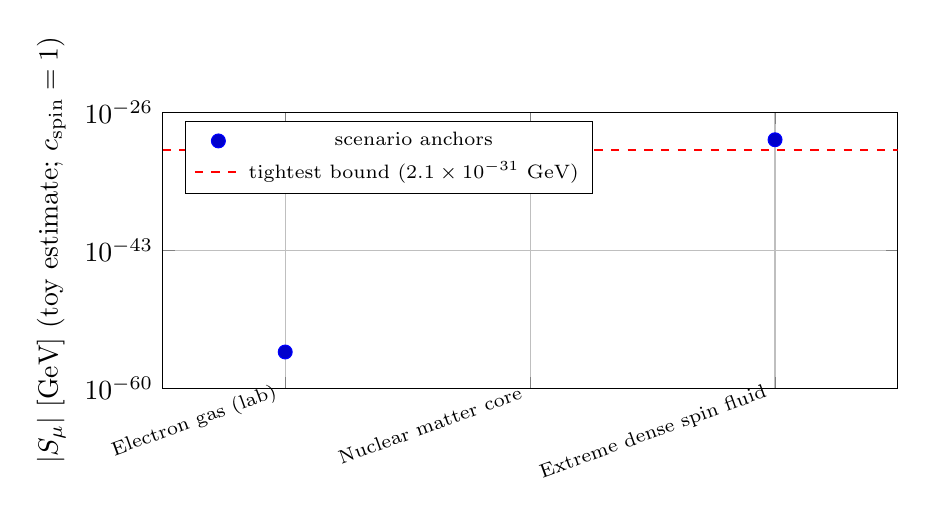
\begin{tikzpicture}
\begin{axis}[
    width=0.9\linewidth,
    height=0.42\linewidth,
    ymode=log,
    ymin=1e-60, ymax=1e-26,
    xmin=0.5, xmax=3.5,
    xtick={1,2,3},
    xticklabels={Electron gas (lab), Nuclear matter core, Extreme dense spin fluid},
    x tick label style={rotate=20, anchor=east, font=\scriptsize},
    ylabel={$|S_\mu|$ [GeV] (toy estimate; $c_{\rm spin}=1$)},
    grid=both,
    legend style={font=\scriptsize},
    legend pos=north west,
]
\addplot+[only marks, mark=*, mark size=2.5pt] coordinates {
    (1,3.2396753580225e-56)
    (2,3.2832238430084956e-31)
    (3,4.104029803760619e-30)
};
\addlegendentry{scenario anchors}

\addplot[red, dashed, thick] coordinates {(0.5,2.1e-31) (3.5,2.1e-31)};
\addlegendentry{tightest bound ($2.1\times10^{-31}$ GeV)}
\end{axis}
\end{tikzpicture}
\caption{Suite regime scan (\texttt{ux\_torsion\_regime\_designer}): torsion estimates and bound-saturation targets across illustrative spin-medium scenarios.}
\end{figure}

%-----------------------------------------------------------------------------
\subsection{Gravitational Coupling from Invariants}
%-----------------------------------------------------------------------------

\begin{corollary}{Gravitational Coupling Consistency}{kappa}
The gravitational coupling $\kappa^2 = 8\pi G$ (with dimension $[\text{energy}]^{-2}$) 
is constrained by consistency with the dimensionless ratio:
\begin{equation}
    \xi \equiv \frac{\cthree}{\phiz}
\end{equation}

\textbf{Dimensional analysis:} Both $\cthree$ and $\phiz$ are dimensionless. The 
physical gravitational coupling $G$ enters when restoring dimensions:
\begin{equation}
    \kappa^2 = 8\pi G = \frac{1}{\Mpl^2}
\end{equation}
The TFPT claim is that the \emph{ratio} $\cthree/\phiz$ is fixed by topology, 
not that $G$ is derived from dimensionless constants alone.

\textbf{Tree-level value:} With $\phitree = 1/(6\pi)$ and $\cthree = 1/(8\pi)$:
\begin{equation}
    \xi_{\text{tree}} = \frac{1/(8\pi)}{1/(6\pi)} = \frac{6\pi}{8\pi} = \frac{3}{4}
\end{equation}

\textbf{With backreaction:} Using $\phiz \approx 0.05317$:
\begin{equation}
    \xi = \frac{0.03979}{0.05317} \approx 0.7483
\end{equation}
This is a shift of $-0.22\%$ from the tree-level value.

\textbf{Physical interpretation:} The ratio $\xi$ determines the relative strength 
of axion-mediated and gravitational interactions. It is \emph{not} a derivation of 
Newton's constant $G$, which remains an input (via $M_{\text{Pl}}$).
\end{corollary}

%=============================================================================
\section{Observable Predictions}
%=============================================================================

%-----------------------------------------------------------------------------
\subsection{Axion--Photon Coupling}
%-----------------------------------------------------------------------------

\begin{corollary}{Axion--Photon Coupling}{gagg}
The CFE fixes the axion--photon vertex uniquely:
\begin{equation}
    \boxed{\gagg = -4\cthree = -\frac{1}{2\pi} \approx -0.1592}
\end{equation}
This determines cosmic birefringence without free parameters.
\end{corollary}

%-----------------------------------------------------------------------------
\subsection{Cosmic Birefringence}
%-----------------------------------------------------------------------------

\begin{definition}{Topological Excursion Quantization}{topoexcursion}
The topological axion excursion is quantized in discrete sector changes:
\begin{equation}
    \Delta a_{\text{top}} = n\,\phiz, \qquad n\in\mathbb{Z},
\end{equation}
with $n=1$ the minimal nontrivial class. The corresponding birefringence is
$\beta = \Delta a_{\text{top}}/(4\pi) = n\,\phiz/(4\pi)$.
\end{definition}

\begin{theorem}{Cosmic Birefringence Prediction}{birefringence}
A homogeneous topological axion field $a_{\text{top}}(\eta)$ rotates the polarization plane of light by:
\begin{equation}
    \frac{d\beta}{d\eta} = 2\cthree\frac{da_{\text{top}}}{d\eta} 
    \quad\Rightarrow\quad 
    \beta = \frac{\Delta a_{\text{top}}}{4\pi}
\end{equation}
Using the coupling convention $\gagg=-4\cthree$ (Corollary~\ref{cor:gagg}) and the sign convention for $\beta$ stated below, the transport law is equivalently
$\frac{d\beta}{d\eta} = -\frac{1}{2}\gagg\,\frac{da_{\text{top}}}{d\eta} = 2\cthree\,\frac{da_{\text{top}}}{d\eta}$.
With the minimal nontrivial sector $n=1$ (Definition~\ref{def:topoexcursion}):
\begin{equation}
    \boxed{\beta_{\text{th}} = \frac{\phiz}{4\pi} = 0.0042312895\ldots~\text{rad} = 0.2424^\circ}
\end{equation}
\end{theorem}

